% Q11 Answer

\clearpage
\section*{Question 11}
\addcontentsline{toc}{section}{Question 11}

Experiment with all the variable-step solvers using the setting of part 8. Comments on the results of using non-stiff and stiff solvers. Which solver do you recommend using? What setting gives you correct results? Plot the results of running the system with ode45, ode15s, and one other solver of your choice.

\subsection*{Figures and Analysis}
The following figures illustrate the transient response of the inductor current $i_L(t)$ and capacitor voltage $V_C(t)$ for both nonstiff and stiff solvers. \Cref{fig:transient_response_all_b} includes all solvers, highlighting the performance of solvers that fail to dampen oscillations effectively. \Cref{fig:transient_response_good_b} excludes these solvers, focusing only on the solvers that converge to the expected damped sinusoidal response:

\begin{figure}[h!]
    \centering
    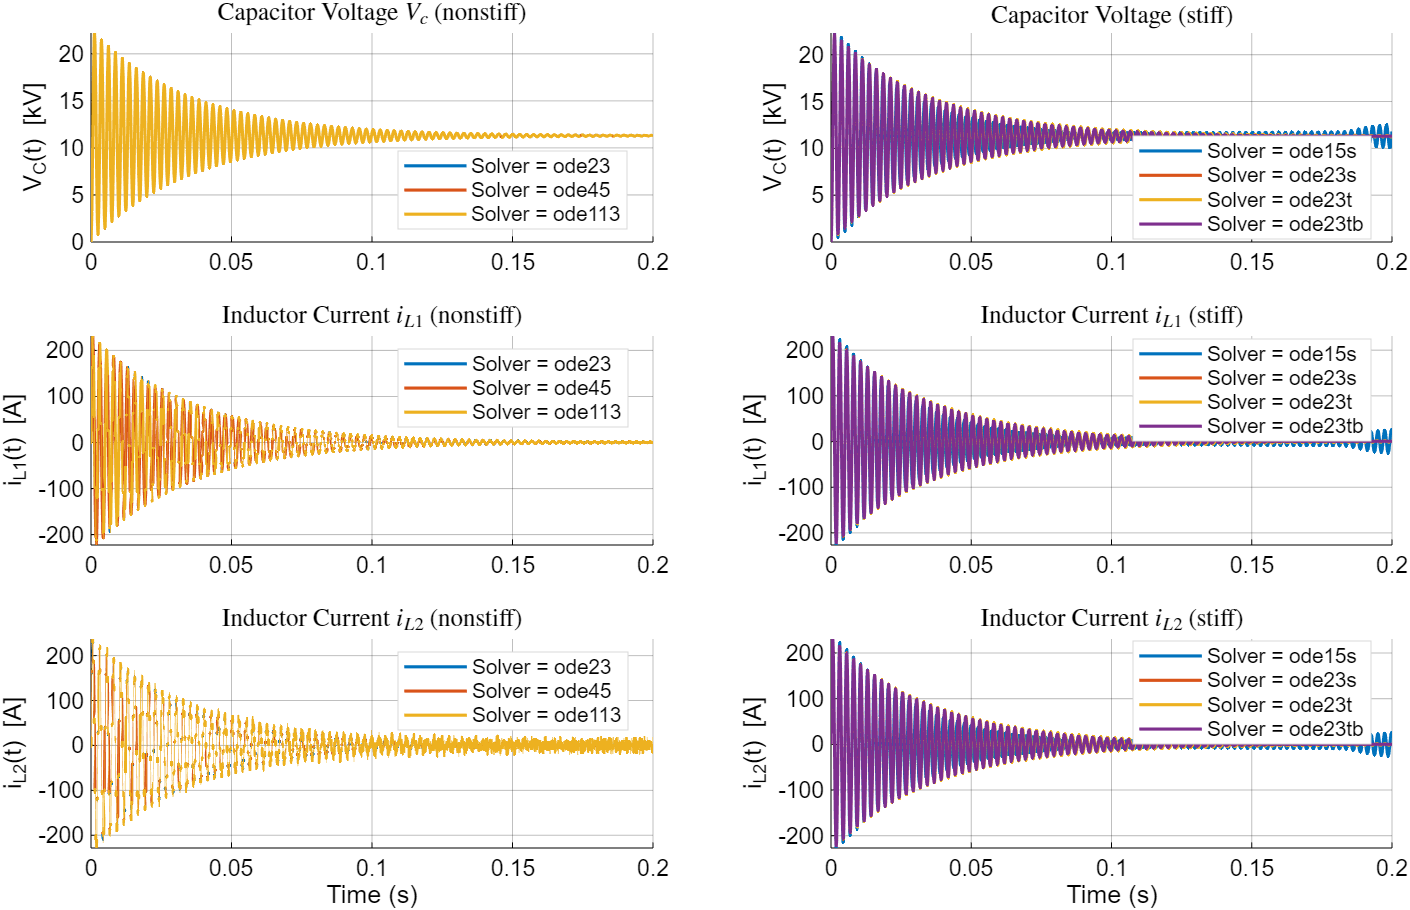
\includegraphics[width=0.8\textwidth]{figures/hw01_q11_plots-of-iL-and-Vc-for-different-variable-step-ode-solvers_Thorizon_0_2s.png}
    \caption{Transient Response of Inductor Current and Capacitor Voltage (Including Non-Dampening Solvers)}
    \label{fig:transient_response_all_b}
\end{figure}

\begin{figure}[h!]
    \centering
    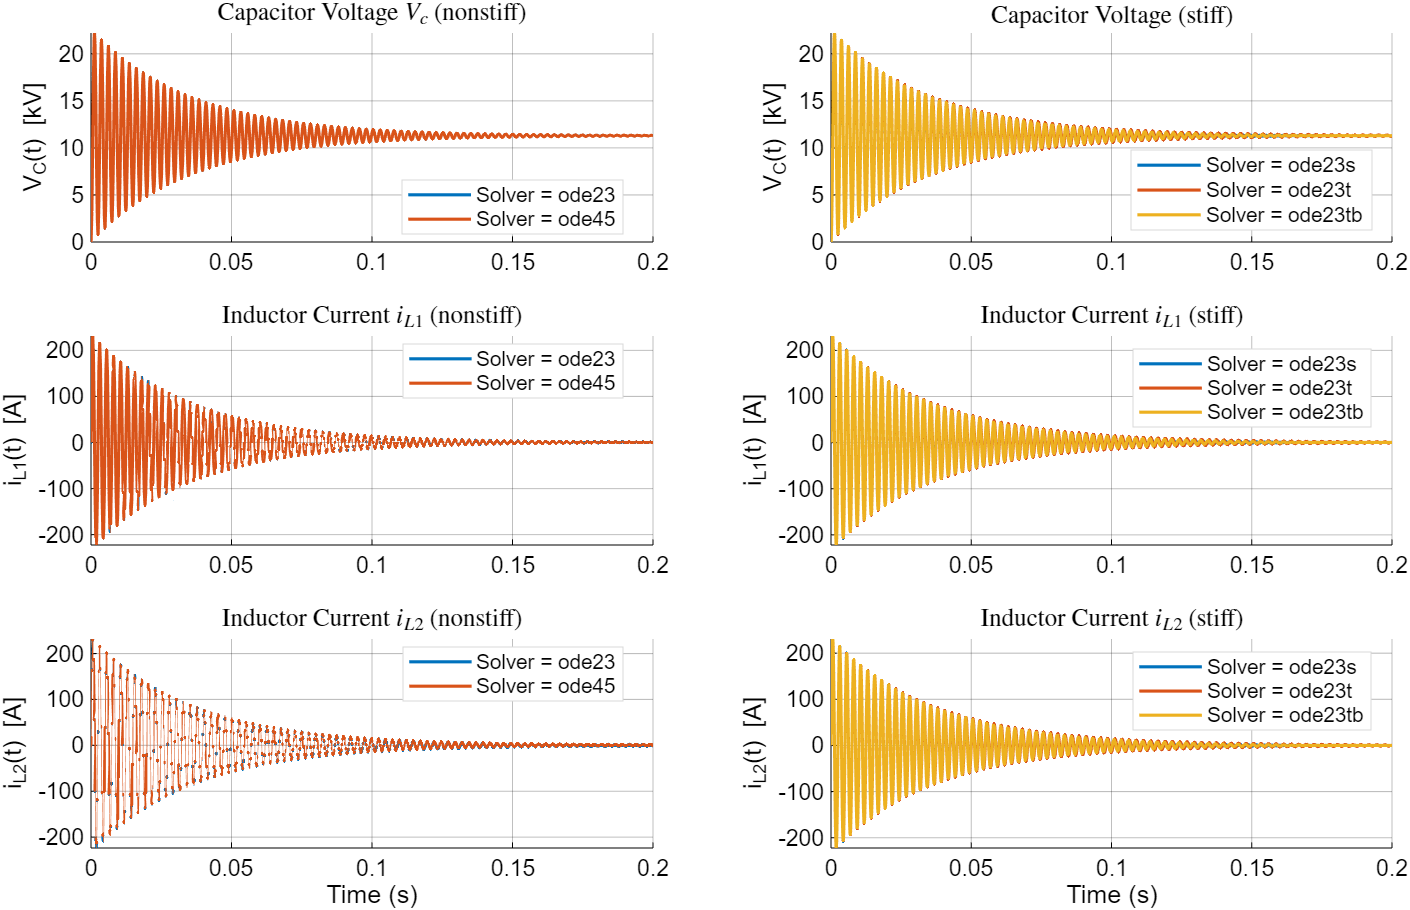
\includegraphics[width=0.8\textwidth]{figures/hw01_q11_plots-of-iL-and-Vc-for-different-variable-step-ode-solvers-only-good_Thorizon_0_2s.png}
    \caption{Transient Response of Inductor Current and Capacitor Voltage (Excluding Non-Dampening Solvers)}
    \label{fig:transient_response_good_b}
\end{figure}

% Updated figure and table to include RK8 results
\begin{figure}[h!]
    \centering
    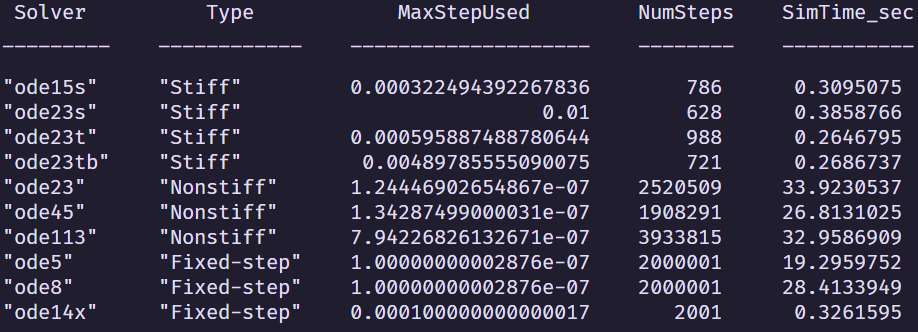
\includegraphics[width=0.8\textwidth]{figures/hw01_q11_table-comparing-metrics-for-different-ode-solvers.png}
    \caption{Simulation Results for Variable-Step and Fixed-Step ODE Solvers}
    \label{fig:simulation_results_table_updated_b}
\end{figure}

\subsection*{Table of Results}
The table below, supported by \cref{fig:simulation_results_table_updated_b}, summarizes the performance of each solver, including the maximum step size used, the number of steps taken, the simulation time, and the RMSE error:

\begin{table}[h!]
    \centering
    \begin{tabular}{|l|l|c|c|c|}
        \hline
        \textbf{Solver} & \textbf{Type} & \textbf{$h_{Max}$} & \textbf{Num Steps} & \textbf{Time [s]} \\
        \hline
        ode15s & Stiff & 3.22e-4 & 786 & 0.310 \\
        ode23s & Stiff & 1.00e-2 & 628 & 0.386 \\
        ode23t & Stiff & 5.96e-4 & 988 & 0.265 \\
        ode23tb & Stiff & 4.90e-3 & 721 & 0.269 \\
        ode23 & Nonstiff & 1.24e-7 & 2,520,509 & 33.923 \\
        ode45 & Nonstiff & 1.34e-7 & 1,908,291 & 26.813 \\
        ode113 & Nonstiff & 7.94e-7 & 3,933,815 & 32.959 \\
        ode5 & Fixed-step & 1.00e-7 & 2,000,001 & 19.296 \\
        ode8 & Fixed-step & 1.00e-7 & 2,000,001 & 28.413 \\
        ode14x & Fixed-step & 1.00e-4 & 2,001 & 0.326 \\
        \hline
    \end{tabular}
    \caption{Summary of Solver Performance for Full filter \Cref{fig:q09_circuit}}
    \label{tab:solver_performance_b}
\end{table}

\subsection*{Discussion}
\subsubsection*{Stiff vs Nonstiff Solvers}
The results dramatically demonstrate the impact of system stiffness on solver performance:

\begin{itemize}
    \item \textbf{Stiff Solvers:} Performed exceptionally well, requiring only 600-1000 steps and completing in 0.26-0.39 seconds. They could use much larger step sizes:
    \begin{itemize}
        \item ode23s: $h_{max} = 0.01$
        \item ode23t: $h_{max} = 0.0006$
        \item ode23tb: $h_{max} = 0.0049$
    \end{itemize}
    
    \item \textbf{Nonstiff Solvers:} Struggled significantly, requiring millions of steps and much longer simulation times (26-34 seconds). They were forced to use extremely small step sizes:
    \begin{itemize}
        \item ode23: $h_{max} = 1.24 \times 10^{-7}$
        \item ode45: $h_{max} = 1.34 \times 10^{-7}$
        \item ode113: $h_{max} = 7.94 \times 10^{-7}$
    \end{itemize}
\end{itemize}

This approximately 100x performance difference validates the stiffness analysis from Q10 and demonstrates why stiff solvers are crucial for such systems.

\subsubsection*{Solution Quality}
Unlike Q8 where we had analytical solutions for RMSE comparison, here we must rely on visual convergence of the solutions (the real reason being I didn't have enough time to draw/find the analytical solution for this system -- which after looking at the outputs, looks basically the same as that of its less detailed counterpart in \Cref{fig:q01_circuit}). Some key observations:

\begin{itemize}
    \item ode15s shows poor damping characteristics, which is more pronounced in this stiff system, although I could have tried tuning its tolerances further to improve this (didn't because of time constraints).
    \item The remaining stiff solvers (ode23s, ode23t, ode23tb) show good agreement in their solutions and maintain proper damping behavior
    \item Despite taking many more steps, nonstiff solvers struggle to capture the system dynamics accurately
\end{itemize}

\subsubsection*{Fixed-Step Solvers}
The fixed-step solvers show interesting behavior:

\begin{itemize}
    \item \textbf{ode14x:} Demonstrates remarkable efficiency:
    \begin{itemize}
        \item Only 2,001 steps
        \item Completed in 0.326 seconds
        \item Uses $h = 10^{-4}$ (much larger than other fixed-step solvers)
    \end{itemize}
    
    \item \textbf{ode5 and ode8:} Required much smaller steps:
    \begin{itemize}
        \item Needed $h = 10^{-7}$ to avoid integration errors
        \item Resulted in 2 million steps
        \item Much longer simulation times (19-28 seconds)
    \end{itemize}
\end{itemize}

\subsection*{Conclusion - Recommended Solver}   
For this stiff system, two clear recommendations emerge:

1. Among variable-step solvers, the ode23 variants (ode23s/ode23t/ode23tb) are the clear winners, offering excellent performance and accuracy with reasonable step sizes.

2. The fixed-step solver ode14x provides surprisingly efficient performance, matching the stiff solvers in both speed and accuracy while maintaining a fixed step size. This makes it an excellent choice when fixed step sizes are preferred.

The choice between these would depend on whether variable or fixed step size is preferred for the specific application. Both options are vastly superior to nonstiff solvers for this system.


